\section{Betriebssysteme}
\subsection{Bare-Metal}
Das Anwender-Programm greift direkt über physikalische Kanäle auf die reale Maschine zu, ist eng mit der realen Maschine gekoppelt und ein einzelner Infinite-Loop (Superloop).

Vorteile: Einfache struktur, nur ein Stack.
Nachteil: Nur schwer Skalierbar

\subsection{Embedded OS}
Das Betriebssystem bildet eine klare Abstraktionsschicht für den Zugriff auf die reale Maschine und entkoppelt die reale Maschine vom Anwender-Programm. Zudem bietet es Anwender-Programmen über logische Kanäle zusätzliche Funktionen und Dienste an.

\subsection{RTOS Kernel}

Besteht aus \textbf{Scheduler}: Algorithmen in jedem Kernel, die bestimmen wann welcher Task ausgeführt wird. Multitasking, z.B. Scheduling-Algorithmen wie Round-Robin, Preemptive Scheduling, etc..

\textbf{Objects}: Kernel-Konstrukte, mit deren Hilfe Entwickler Anwendungen für Real-Time Embedded Systems
erstellen können (z.B. für IPC, Synchronisation). z.B. Tasks, Semaphores, Message Queues, etc..

\textbf{Services}: z.B. Timing, Interrupt Handling, Resource Management wie File System, etc., weitere Operationen des Kernels auf einem Object.

\subsection{betriebsystem Architekturen}

\begin{minipage}[t]{.45\linewidth}
	\centering
	Monolithische Architektur

	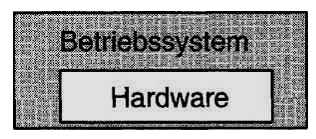
\includegraphics[width=.8\textwidth]{os_architektur_monolithisch.png}
\end{minipage}\hfill
\begin{minipage}[t]{.45\linewidth}
	\centering
	Kern-Schale Architektur

	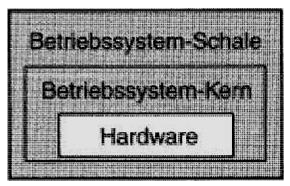
\includegraphics[width=.8\textwidth]{os_architektur_kernschalen.png}
\end{minipage}

\begin{minipage}[t]{.45\linewidth}
	\centering
	Hierarchische Schichten

	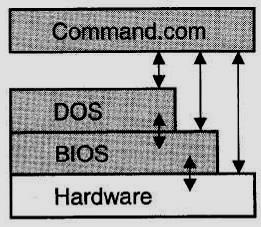
\includegraphics[width=.8\textwidth]{os_architektur_hirarchisch.png}
\end{minipage}\hfill
\begin{minipage}[t]{.45\linewidth}
	\centering
	Mikrokern

	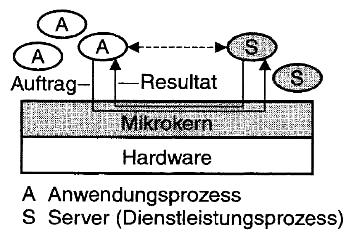
\includegraphics[width=\textwidth]{os_architektur_mikrokern.png}
\end{minipage}

\begin{minipage}[t]{\linewidth}
	\centering
	Virtuelle Maschine

	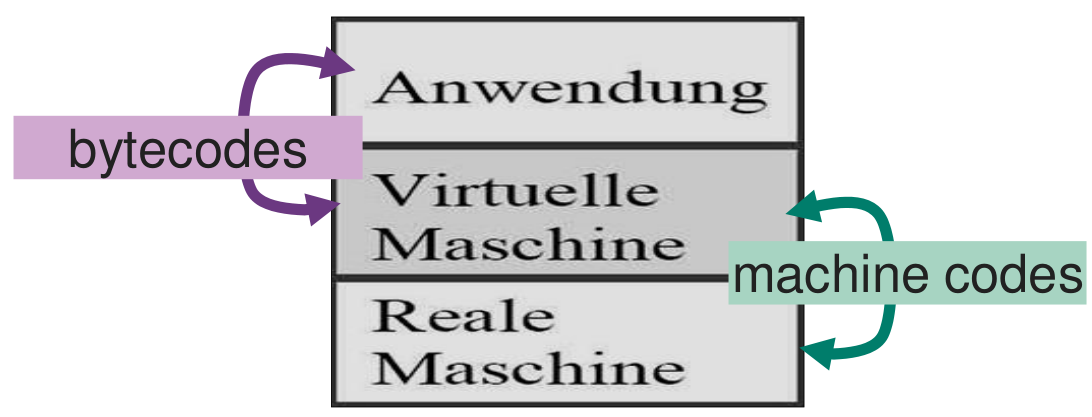
\includegraphics[width=.6\textwidth]{os_architektur_virtuellemaschiene.png}
\end{minipage}


\section{FreeRTOS}

\subsection{Tasks und Scheduling}

\begin{center}
	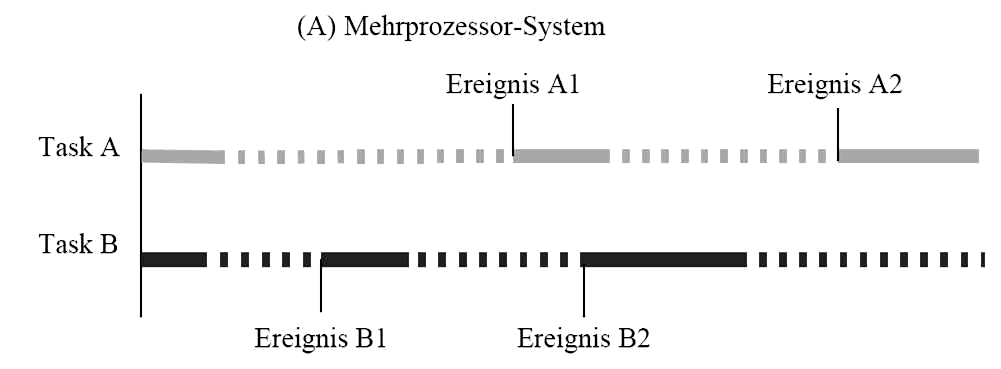
\includegraphics[width=.8\linewidth]{quasi_parallel_mehrprozessor.png}
\end{center}

Sehr aufwändig. Multiprocessing, Multithreading.

\begin{center}
	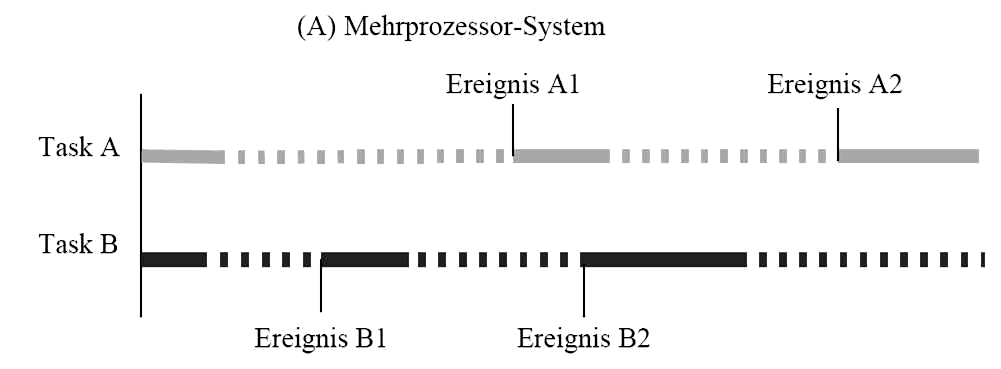
\includegraphics[width=.8\linewidth]{quasi_parallel_mehrprozessor.png}
\end{center}

Multitasking.

\subsection{Parallele Prozesse}
\subsubsection{Prozessmodell vs. Threadmodell}
Das Threadmodell ist typisch bei eingebetteten Systemen (Embedded OS, RTOS). Unterscheiden bei den Kontextgruppen.

\begin{minipage}[t]{.49\linewidth}
	Prozessmodell

	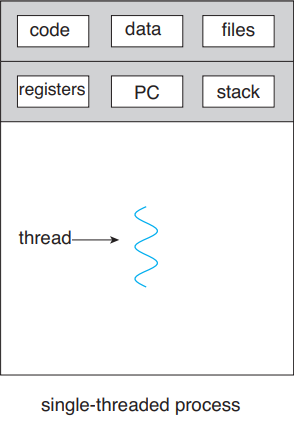
\includegraphics[height=5cm]{prozessmodell.png}
\end{minipage}\hfill
\begin{minipage}[t]{.49\linewidth}
	Threadmodell

	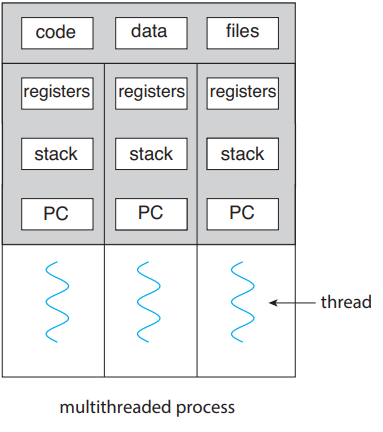
\includegraphics[height=5cm]{threadmodell.png}
\end{minipage}

\subsubsection{Prozesszustände}

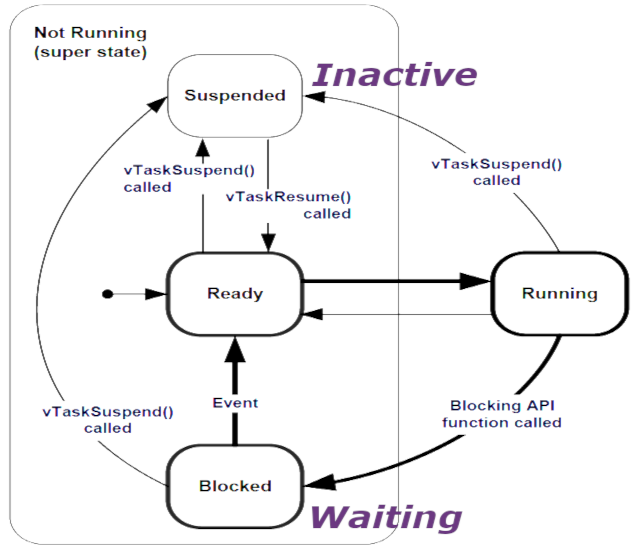
\includegraphics[width=\linewidth]{prozesszustaende.png}

Siehe auch Abschnitt \ref{sec:task_management}.

Das Betriebssystem verwaltet mehrere Warteschlangen, welche typischerweise als Linked List implementiert werden:

\begin{itemize}
	\itemsep-.5em
	\item \textit{Ready-Queue}: Enthält die lauffähigen Prozesse. Auch mehrere Ready-Listen können vorhanden sein, z.B. eine pro Prioritätsstufe.
	\item \textit{Waiting-Queues}: Für sämtliche unterscheidbaren Warte-Ereignisse wird je nach Ereignistyp eine eigene Queue geführt.
\end{itemize}


\subsection{Scheduling und Context Switch}

Ein Prozesswechsel führt im Betriebssystem zu folgende Aktionen:

\begin{enumerate}
	\itemsep-.5em 
	\item Sicherung des gesamten Kontexts vom unterbrochenen Prozess 1.
	\item Änderung des Zustands von Prozess 1 zu \textit{Ready} oder \textit{Waiting} (je nach Grund der Unterbrechung).
	\item Auswahl des zu aktivierenden Prozesses 2 durch den Scheduler.
	\item Änderung des Zustands von Prozess 2 von \textit{Ready} zu \textit{Running}.
	\item Wiederherstellung des (gesicherten) Kontexts von Prozess 2. Durch Laden der Prozessorregister wird dieser Prozess nun fortgesetzt.
\end{enumerate}

Wenn beim Scheduling kein anderer Prozess laufbereit ist, wird der \textbf{Idle Task} aufgerufen, welcher meist nur aus einer Warteschleife besteht.
Ohne den Idle Task müsste innerhalb des Betriebssystem-Kerns gewartet werden ("busy waiting").

Das \textbf{Kernsperren} verhinder ungewollte Interrupts.

\subsubsection{Scheduling-Strategien}

\begin{itemize}
	\itemsep-.5em 
	\item CPU-Auslastung (CPU utilization), Ziel ist 100\% Auslastung der CPU.
	\item Durchsatz (throughput), Anzahl erledigter Tasks pro Zeiteinheit.
	\item Faire Behandlung (fairness), Kein Task soll bevorzugt werden.
	\item Ausführungszeit (turnaround time), Zeitspanne von Beginn bis Ende des Tasks.
	\item Wartezeit (waiting time), Ziel, die Wartezeiten zu minimieren.
	\item Antwortzeit (response time), Ziel, Antwortzeit zwischen Eingabe und resultierender Reaktion zu minimieren.
\end{itemize}

Scheduling-Konfiguration in \lstinline[style=cppstyle]|FreeRTOSConfig.h|.

\begin{itemize}
	\itemsep-.5em 
	\item Preemptive:	Task mit höchster Priorität ausgeführt; Tasks gleicher Priorität teilen CPU-Zeit (Round Robin);	optionales Time Slicing
	\item Cooperative:	Kontextwechsel (Task Switch) nur falls Task blockiert, oder bei explizitem \lstinline[style=cppstyle]|taskYIELD();|. Prozess läuft solange, bis er die CPU selber freigibt.
\end{itemize}

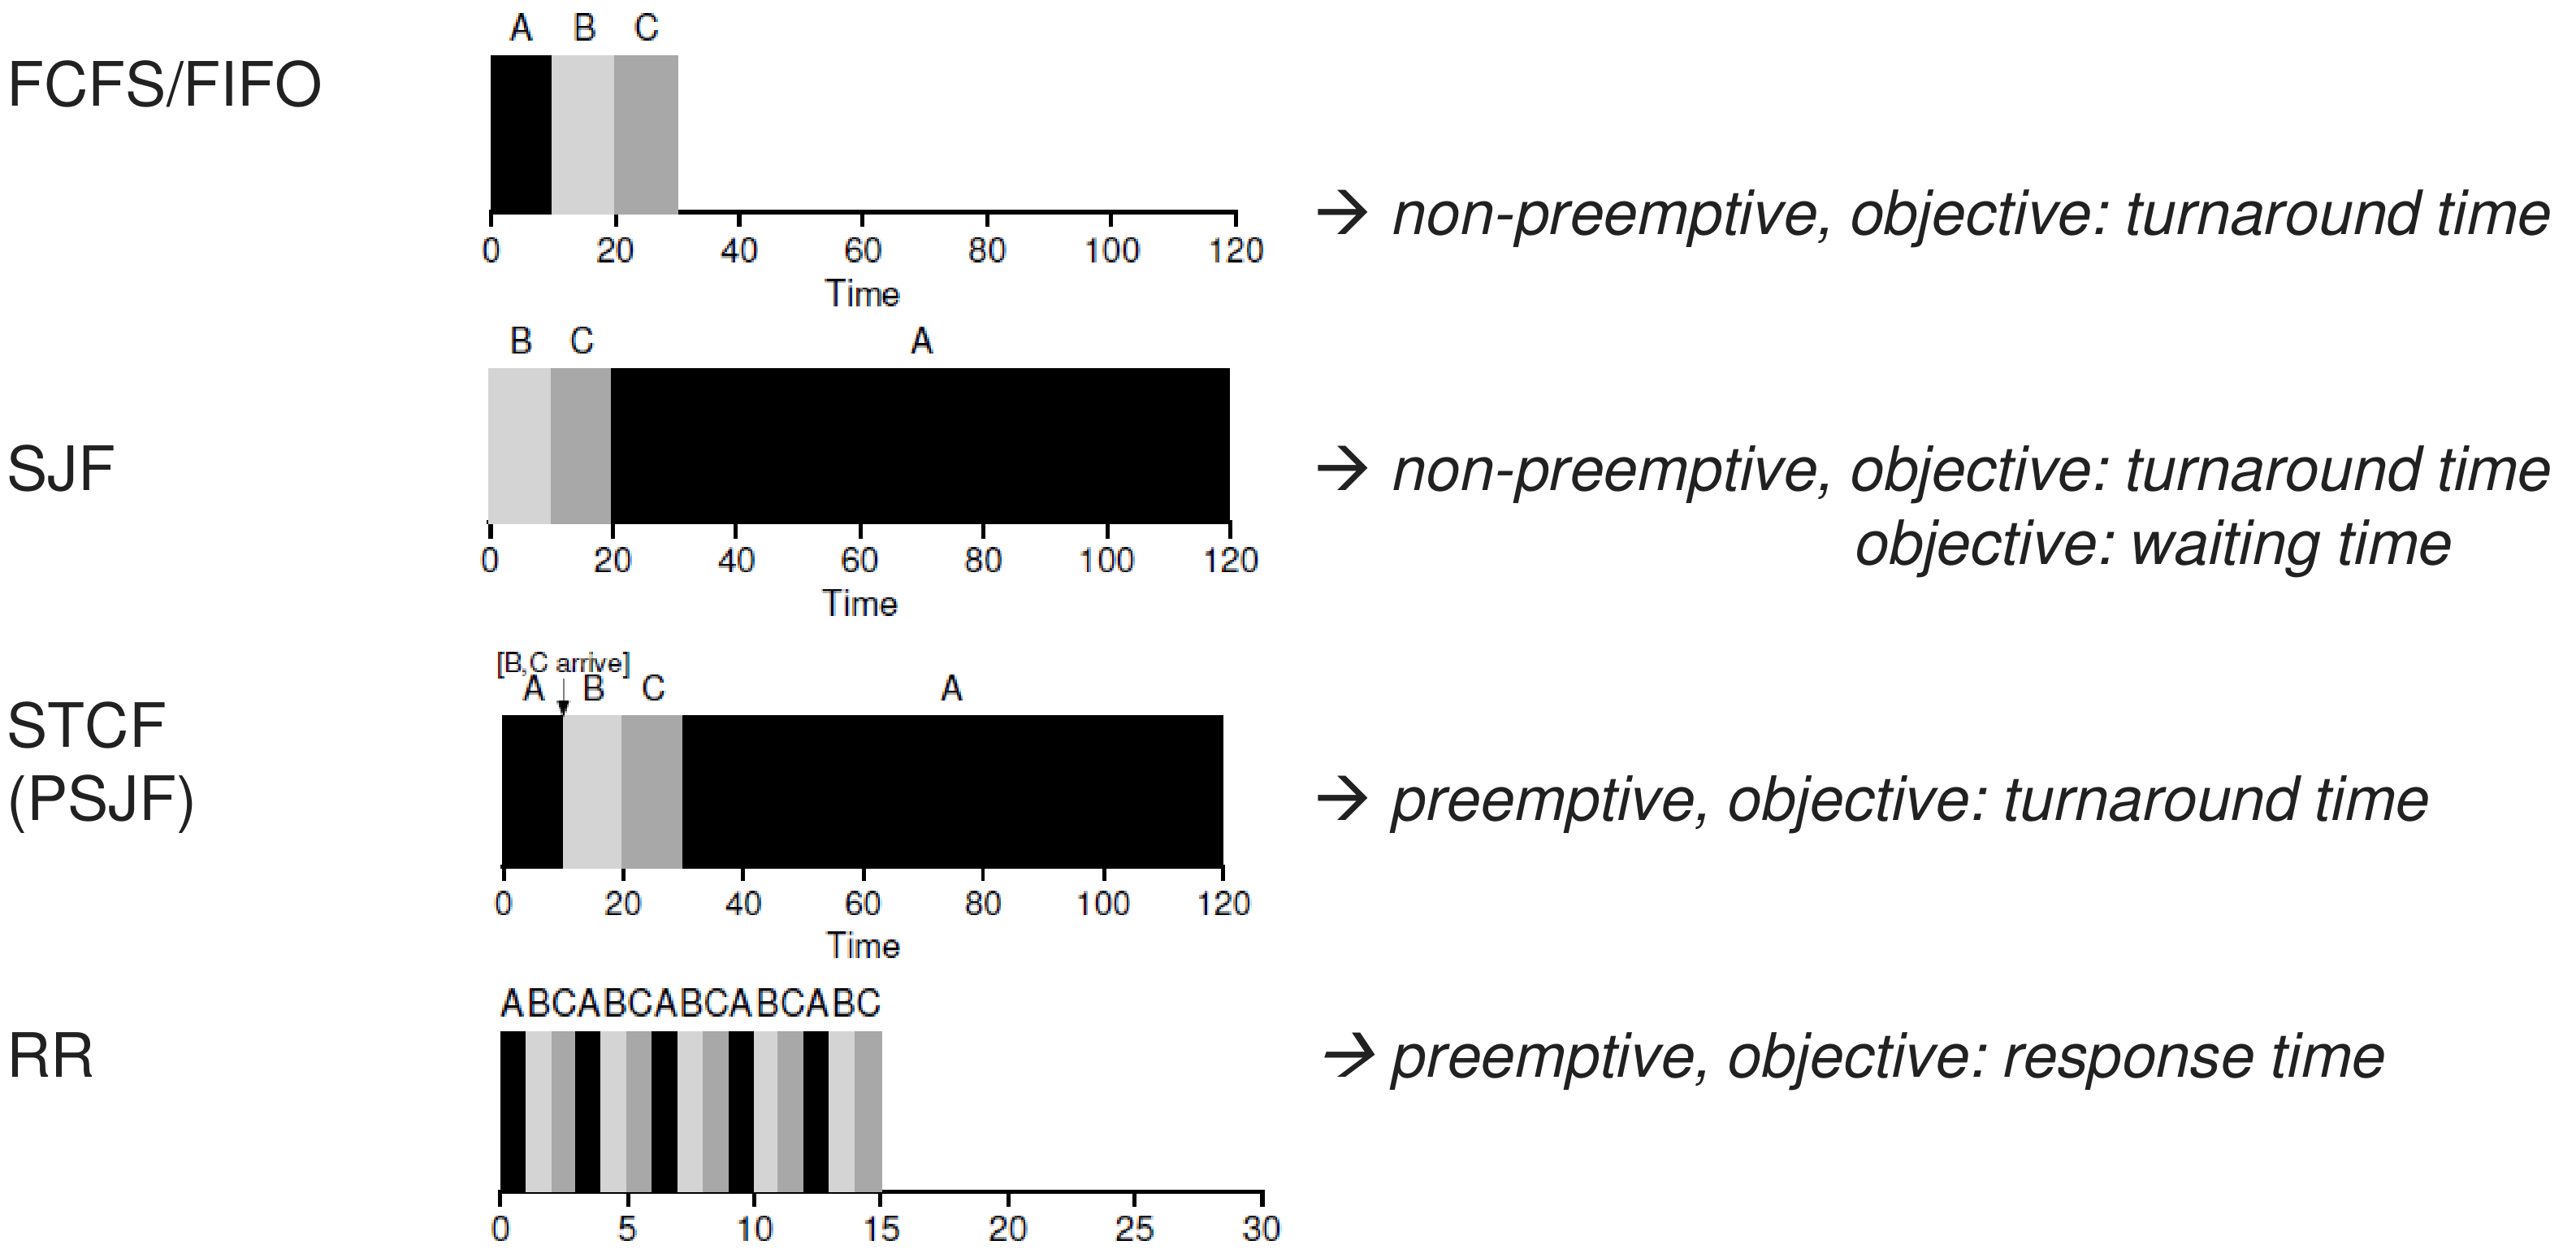
\includegraphics[width=\linewidth]{Scheduling_Strategien.png}

